\section{分部积分}
\label{sec:mcalc-integration-by-parts}

一元的分部积分
\[
\int_a^bf\,q'\,\mathrm dt=\bigl[fq\bigr]_a^b-\int_a^bf'q\,\mathrm dt
\]
把导数从一个因子移到另一个因子，代价是一个边界项。这就是Stokes公式的最简单形式。流形上，散度定理扮演微积分基本定理的角色，梯度与散度扮演一对“互为转置”的导数：类比矩阵的转置把$\bm x^\top\bm A\bm y$中的$\bm A$移到另一侧，分部积分把导数从一个函数移到另一个函数，在$L^2$内积下二者互为负转置。

本节先把二者组织成分部积分公式，再区分边界项在什么条件下消失，最后说明这一公式怎样成为弱导数与场方程的接口。

\paragraph{乘积规则与分部积分公式}
分部积分的出发点是散度的乘积规则：对光滑函数$f$与向量场$X$，
\begin{equation}
\operatorname{div}(fX)=f\operatorname{div}X+g(\operatorname{grad}f,X).
\label{eq:mcalc-divergence-product}
\end{equation}
它由定义直接得到：协变导数满足$\nabla_{\bm v}(fX)=(\bm vf)X+f\nabla_{\bm v}X$，取迹时第二项给出$f\operatorname{div}X$，第一项是线性映射$\bm v\mapsto\mathrm df(\bm v)X$的迹，等于$\mathrm df(X)=g(\operatorname{grad}f,X)$。

\begin{theorem}[分部积分公式]
\label{thm:mcalc-integration-by-parts}
设$(M,g)$是带边界的黎曼流形，$N$是外单位法向，$f\in C^\infty(M)$，$X\in\mathfrak X(M)$，并且$fX$有紧支撑。则
\begin{equation}
\int_Mf\,\operatorname{div}X\,\mathrm dV_g=-\int_Mg(\operatorname{grad}f,X)\,\mathrm dV_g+\int_{\partial M}f\,g(X,N)\,\mathrm dA .
\label{eq:mcalc-integration-by-parts}
\end{equation}
\end{theorem}

\begin{proof}
对紧支撑的向量场$fX$应用定理~\ref{thm:mcalc-divergence-theorem}，得到
\[
\int_M\operatorname{div}(fX)\,\mathrm dV_g=\int_{\partial M}f\,g(X,N)\,\mathrm dA .
\]
再把式~\eqref{eq:mcalc-divergence-product}代入左端并移项。各项积分都有限，因为被积函数连续且支撑含于$fX$的紧支撑中。
\end{proof}

取$X=\operatorname{grad}q$，记法向导数$\partial_Nq=\mathrm dq(N)$，由$g(\operatorname{grad}q,N)=\partial_Nq$，得到Green第一恒等式
\begin{equation}
\int_Mf\,\Delta_gq\,\mathrm dV_g=-\int_Mg(\operatorname{grad}f,\operatorname{grad}q)\,\mathrm dV_g+\int_{\partial M}f\,\partial_Nq\,\mathrm dA .
\label{eq:mcalc-green-identity}
\end{equation}
交换$f,q$再相减，梯度内积项抵消，得到Green第二恒等式：两个Laplace--Beltrami积分之差只剩边界项，
\begin{equation}
\int_M(f\,\Delta_gq-q\,\Delta_gf)\,\mathrm dV_g=\int_{\partial M}(f\,\partial_Nq-q\,\partial_Nf)\,\mathrm dA .
\label{eq:mcalc-green-second}
\end{equation}
这两个等式统称\term{Green恒等式}（Green's identities）。

用上半球面$M$上的高度函数核对边界项。取$f\equiv1$、$q=h$，$\partial M$是赤道，赤道上$N=-\bm e_3$，$\operatorname{grad}h=\bm e_3$，所以$\partial_Nh=-1$。式~\eqref{eq:mcalc-green-identity}右端的梯度项因$\operatorname{grad}1=0$消失，边界项为$-2\pi$，于是应有$\int_M\Delta_gh\,\mathrm dV=-2\pi$。

直接计算左端，用$\Delta h=-2h$与$h=\cos\theta$，
\[
\int_M(-2\cos\theta)\sin\theta\,\mathrm d\theta\,\mathrm d\phi=-2\cdot2\pi\int_0^{\pi/2}\cos\theta\sin\theta\,\mathrm d\theta=-2\pi ,
\]
两端相等。

\paragraph{边界项何时消失}
边界项是否出现，决定了$\Delta_g$能否像对称矩阵那样“自由转置”。常见的有三种情形，所依据的条件各不相同。
\begin{enumerate}
\item \emph{闭流形}，即紧且无边界的流形，例如球面和环面。此时$\partial M=\varnothing$，紧性使任何光滑函数都紧支撑，式~\eqref{eq:mcalc-green-identity}的边界项不出现，$\Delta_g$在$L^2$内积下关于$f,q$对称。
\item \emph{紧支撑}，即$f$或$q$在边界附近为零且支撑紧。这是非紧流形上最常用的条件，本节末尾定义弱导数时的试验函数就取这一类。
\item \emph{边界条件}。在紧的带边界流形上，若$f$在$\partial M$上为零（Dirichlet条件），第一恒等式的边界项消失；若$\partial_Nq=0$（Neumann条件），同样消失。第二恒等式中的边界项要求两个函数满足同一类条件才全部消失。
\end{enumerate}

在闭流形上取$f=q$，得到
\begin{equation}
\int_Mq\,\Delta_gq\,\mathrm dV_g=-\int_M\lVert\operatorname{grad}q\rVert_g^2\,\mathrm dV_g\leq0 ,
\label{eq:mcalc-laplacian-nonpositive}
\end{equation}
这就是上一节所说$\Delta_g$“非正”的含义。若$\Delta_gq=0$（称$q$为调和函数），则$\operatorname{grad}q\equiv0$；在连通的闭流形上，梯度为零的函数沿任何曲线导数为零，因而是常数。所以连通闭流形上的调和函数只有常数。

用单位球面上的高度函数验证式~\eqref{eq:mcalc-laplacian-nonpositive}。左端用$\Delta h=-2h$，
\[
\int_{S^2}h\,\Delta h\,\mathrm dV=-2\int_{S^2}h^2\,\mathrm dV=-2\cdot2\pi\int_0^\pi\cos^2\theta\sin\theta\,\mathrm d\theta=-\frac{8\pi}3 .
\]
右端由$\lVert\operatorname{grad}h\rVert_g=\sin\theta$，
\[
-\int_{S^2}\sin^2\theta\,\mathrm dV=-2\pi\int_0^\pi\sin^3\theta\,\mathrm d\theta=-\frac{8\pi}3 ,
\]
两端相等，也都为负。

\paragraph{非紧时不能省略条件}
在无边界但非紧的流形上，即使没有边界，边界项也可能“藏在无穷远处”。取$M=\mathbb R$，$f\equiv1$，$X=\tanh(x)\,\partial_x$。这时左端是
\[
\int_{\mathbb R}\operatorname{div}X\,\mathrm dx=\int_{\mathbb R}\operatorname{sech}^2x\,\mathrm dx=\tanh(+\infty)-\tanh(-\infty)=2 .
\]
而右端的梯度项因$\operatorname{grad}f=0$为零，又没有边界，式~\eqref{eq:mcalc-integration-by-parts}的两端不等。

\begin{BookInlineFigure}
  \centering
  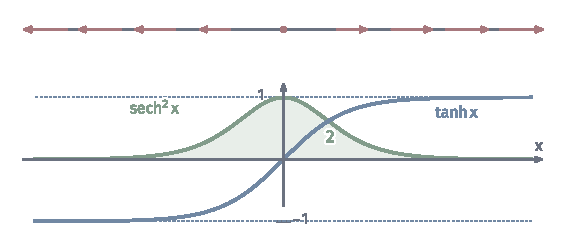
\includegraphics[width=96mm]{figures/04-spaces-measures-and-geometry/04-manifolds/matplotlib/mcalc-noncompact-flux/figure.pdf}
  \caption{$M=\mathbb R$上的$X=\tanh(x)\,\partial_x$。上方的红箭头是向量场本身，两端趋于$\pm\partial_x$。下方绿线是散度$\operatorname{sech}^2x$，浅绿面积为$2$；蓝线是$X$的分量$\tanh x$，它在两端趋于$\pm1$，这两个极限恰是逃向无穷远的流量。}
  \label{fig:mcalc-noncompact-flux}
\end{BookInlineFigure}

问题在于$fX$没有紧支撑。图~\ref{fig:mcalc-noncompact-flux}上方的箭头显示，流量一直流向无穷远，散度的累计$2$由这两股流量解释。非紧情形要使用分部积分，须验证紧支撑，或者验证被积函数衰减得足够快，使截断后边界项的极限为零。

\paragraph{弱导数与场方程的接口}
式~\eqref{eq:mcalc-integration-by-parts}对紧支撑的$f$不含边界项，可以反过来用作定义。第~\ref{chap:smoothing-weak-derivatives}章在欧氏开集上，用与紧支撑试验函数的积分关系定义弱导数。流形上同样可以说：局部可积的向量场$Y$是函数$u$的弱梯度，若对所有紧支撑于$M$内部的光滑向量场$X$，
\begin{equation}
\int_Mu\,\operatorname{div}X\,\mathrm dV_g=-\int_Mg(Y,X)\,\mathrm dV_g .
\label{eq:mcalc-weak-gradient}
\end{equation}
对光滑的$u$，$Y=\operatorname{grad}u$满足这一式；对不光滑的$u$，它在不求导的前提下刻画了“梯度”。

看圆周上的例子。取$S^1$的角度坐标$\theta\in(-\pi,\pi]$，度量$\mathrm d\theta^2$，$u(\theta)=\lvert\theta\rvert$。$u$在$\theta=0$与$\theta=\pm\pi$处有折点，不是$C^1$函数。对周期的光滑函数$X$，在$(-\pi,0)$与$(0,\pi)$上分别分部积分，
\[
\int_{-\pi}^{\pi}\lvert\theta\rvert X'\,\mathrm d\theta=\pi X(\pi)-\pi X(-\pi)-\int_0^\pi X\,\mathrm d\theta+\int_{-\pi}^0X\,\mathrm d\theta .
\]
边界项因$X$的周期性相消，于是$u$有弱梯度$Y=\operatorname{sgn}(\theta)\,\partial_\theta$。在$\theta=0$处，两侧的边界项因$u$连续而相消，所以折点不妨碍弱导数存在；若函数在某点跳跃，这样的项就消不掉，第~\ref{chap:smoothing-weak-derivatives}章已讨论过这种差别。

同理，方程$\Delta_gu=s$的弱形式是：对所有紧支撑的光滑$\varphi$，
\begin{equation}
-\int_Mg(\operatorname{grad}u,\operatorname{grad}\varphi)\,\mathrm dV_g=\int_Ms\varphi\,\mathrm dV_g ,
\label{eq:mcalc-weak-laplace}
\end{equation}
它只要求$u$有一阶弱导数。下一节的Sobolev空间为这些弱形式提供函数类，而弱解的存在、唯一与边值问题可参考\BookChapterRef{chap:elliptic-equations}{卷六第4章“椭圆方程与边值问题”}。
